\documentclass[11pt]{article}
\usepackage{latexsym}
\usepackage{amssymb,amsmath}
\usepackage[pdftex]{graphicx}
% \usepackage{qtree}

\topmargin = -.75in \textwidth=7in \textheight=9.3in
\oddsidemargin = -.3in \evensidemargin = -.3in

\begin{document}
\begin{center}
\large
CS181 Assignment 1
\end{center}
Joy Ming and Alisa Nguyen (9 February 2013)\\

\begin{enumerate}
\setcounter{enumi}{0}

\item Decision Trees and ID3
\begin{enumerate}
\item ID3 will chose to split on \fbox{A} because it has a higher information gain.
	\begin{itemize}
	\item Splitting on A will have an information gain of $Gain(X_k,A)=H(A)-Remainder(X_k,A)=$ \fbox{0.025}, 
		where $H(A) = \frac{3}{7}\log_2 \frac{7}{3} + \frac{4}{7}\log_2\frac{7}{4}=0.985$, % Not sure about this part sorry
		and $Remainder(X_k,A)=\frac{4}{7}(\frac{2}{4}\log_2 2+\frac{2}{4}\log_2 2+\frac{3}{7}(\frac{2}{3}\log_2 \frac{3}{2} + \frac{1}{3}\log_2 3) = 0.96$
	\item Splitting on B will have an information gain of $Gain(X_k,B)=H(B)-Remainder(X_k,B)=$ \fbox{0.005}, 
		where $H(B) = \frac{4}{7}\log_2 \frac{7}{4} + \frac{2}{7}\log_2\frac{7}{2}=0.985$, % Not sure about this part sorry
		and $Remainder(X_k,B)=\frac{2}{7}(\frac{1}{2}\log_2 2+\frac{1}{2}\log_2 2+\frac{5}{7}(\frac{3}{5}\log_2 \frac{5}{3} + \frac{2}{5}\log_2 \frac{5}{2})=0.98$
	\end{itemize}
This example shows that ID3 has an inductive bias of strongly preferring extreme partitions and larger subsets. In this case, looking at the results of the of when both A and B are true, they have the same 1:1 ratio of positive and negative outputs, but A is preferred because it has two data points for each whereas B only has one. IS THIS TRUE??
\item In this example, a tree that could be formed would split first on A, then B, then C, as shown below.\\
	$$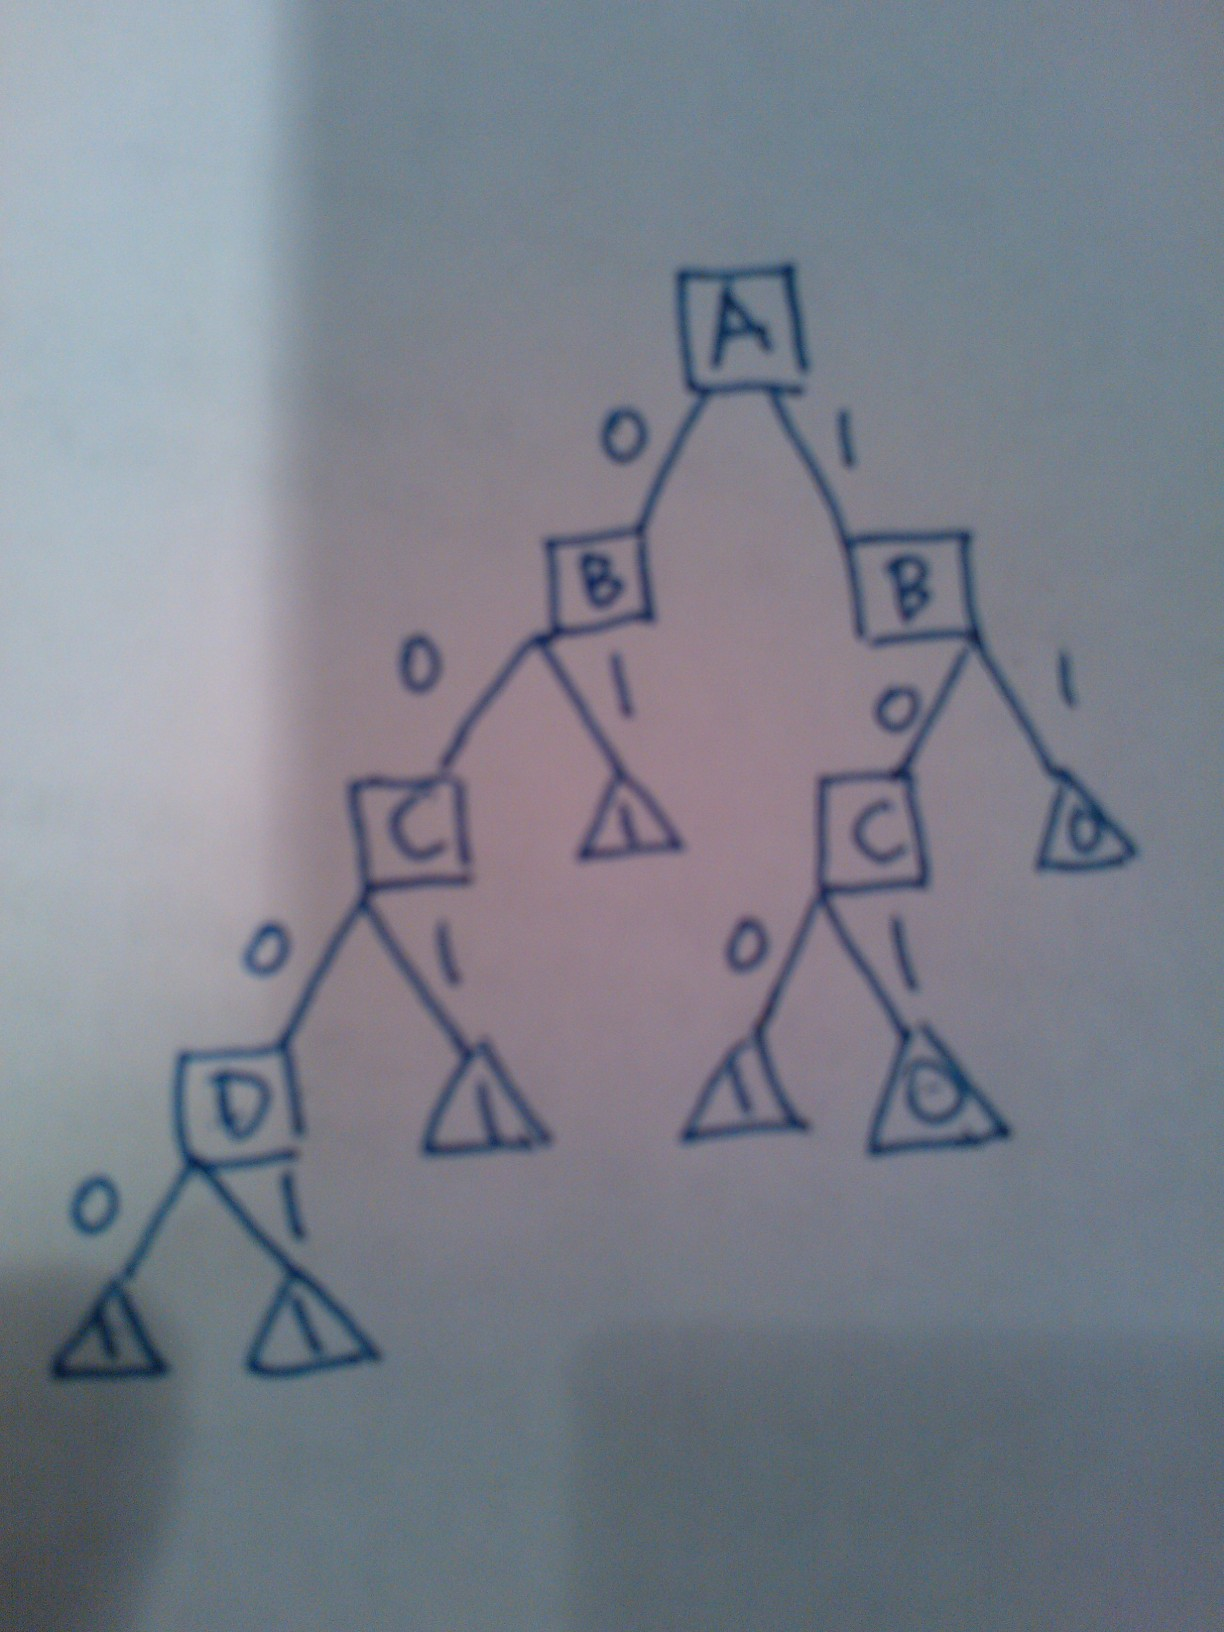
\includegraphics[width=80mm]{Q1PB.jpg}$$
	\\This tree splits first at A, without a tie.
	\\ Then following A = 1, both B and C have the same information gain so we split on B to proceed alphabetically. 
	\begin{itemize}
	\item Where B = 1 there is only one output, Label = 0, so we return a leaf.  
	\item Where B = 0 there are different outputs so we split on C, which returning two leaves: when C = 1, Label = 0 and when C = 0, Label = 1. 
	\end{itemize}
	Following A = 0, both B and C have same information gain, and we split on B for the same reasons as above (simple alphabetical ordering). 
	\begin{itemize}
	\item When B = 1, there is only one value for Label, or Label = 1. 
	\item When B = 0, we are left with an even Label split which cannot be resolved by either C or D. We don't split on C because it has the same split as B so it will have a 0 information gain. We also don't split on D because for the cases where B = 0, it has the same labels and does not contribute more information. So we return the majority Label, or Label = 1.
	\end{itemize}
% \Tree [.A [.0 [.B [.0 [.C [.0 ?] [.1 ?]]] [.1 .1]]] [.1 [.B [.0 [.C [.0 .1] [.1 .1]]] [.1 [??]]]]]
% Does the tree compile on your computer? 
\item By eyeballing the data and looking for the sources of error, a simpler decision tree that has the same training error would be one where the A=0 branch does not split, rather, just returns a Label = 1 leaf. This can be seen first by looking at the A=0 and B = 0 branch, which splits on D into two leaves which both have Label = 1, which is redundant. However, since both of these leaves were determined using different manners (one from the data, one by taking the majority value), the algorithm does not know it is being redundant. In this case, the subtree that is splitting by D can just be replaced by a leaf Label = 1. Then looking at the B split on the A = 0 branch we see that it also has the same leaf values, which is, once again, redundant. Therefore, we can condense these into a single leaf Label = 1. This is a simpler tree that has the same training error as the original one created by the ID3 algorithm. From this example we can learn that the ID3 algorithm has inductive bias, especially because it is greedy and only chooses the single attribute with the highest information gain. It does not look back to see if what it did was necessary or statistically significant. What we did to find the simpler tree is along the lines of the logic of post-pruning--checking to see if the split was necessary and changing it.
\end{enumerate}

\item ID3 with Pruning
\begin{enumerate}
\item The average cross-validated training performance was:
	\begin{itemize}
	\item Non-noisy: Training \fbox{1.0} and test \fbox{0.87}.
	\item Noisy: Training \fbox{0.98} and test \fbox{0.78}.
	\end{itemize}
\item After the pruning function:
	\begin{enumerate}
	\item $$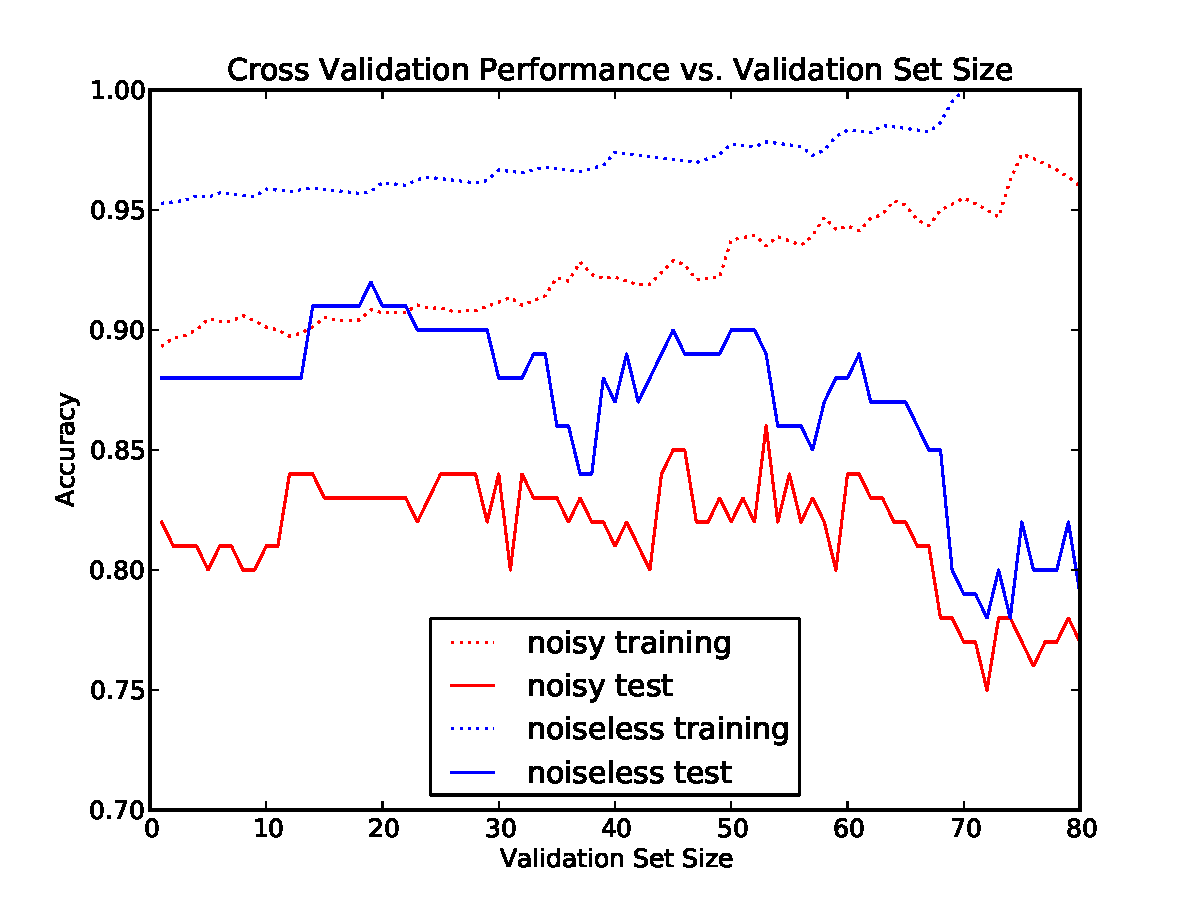
\includegraphics[width=150mm]{nguyen-ming-2bi.pdf}$$
	\item The cross-validated performance of the validation set pruning improves at first, as the valdiation increases from 1, peaks at a point around size 40 to 60, and then worsens in performance as the validation set size becomes too large and overfitting becomes an issue.
	\item The validation set pruning improves the cross-validated performance of ID3 on these data for all the data points leading up to the peak when comparing against validation-size. After the peak, pruning gives us similar and sometimes slightly worse results than the cross-validated performance of ID3. On the nosy data, the average cross-validated test perfromance with pruning on the non-noisy dataset is 0.8599 and without pruning 0.855.
	\item Overfitting is an issue for these data, as evidenced by the dropoff after a peak when the validation set size gets too large. ELABORATE.
	\end{enumerate}
\end{enumerate}

\item Boosting
\begin{enumerate}
	\item The weighted entropy of the set can be calculated:\\
	$W=0.5 + \frac{0.5}{N-1}(N-1) = 1$
	$H = 0.5\log_2 \frac{1}{0.5} + 0.5\log_2 \frac{1}{0.5} =$ \fbox{1}
	\begin{enumerate} 
	\item Analyze the effectiveness of boosting:
		\begin{enumerate}
			\item Effect of maximum depth on cross validated boosting in noisy(Y) and noise-less(N) data
				\begin{center}
				\begin{tabular}{|c|c|c|c|}
				\hline
				Noisy? & Max depth & $R = 10$ & $R = 30$\\ \hline
				Y & 1 & 0.82 & 0.84\\ \hline
				N & 1 & 0.89 & 0.91\\ \hline
				Y & 2 & 0.81 & 0.79 \\ \hline
				N & 2 & 0.87 & 0.87\\
				\hline
				\end{tabular}
				\end{center}
			For each given set of data that is the same noisyness and number of rounds, it seems the greater the maximum depth the less accurate the created learner is. This is in part because the bigger the tree, the less of a "weak" learner it is. In this example, the greater the depth the more splits the tree will go through and thus will create a higher probabilitiy of overfitting. NEEDS MORE BUZZ WORDS
			\item Effect of number of boosting rounds on cross-validated performance of decision trees:\\
			 $$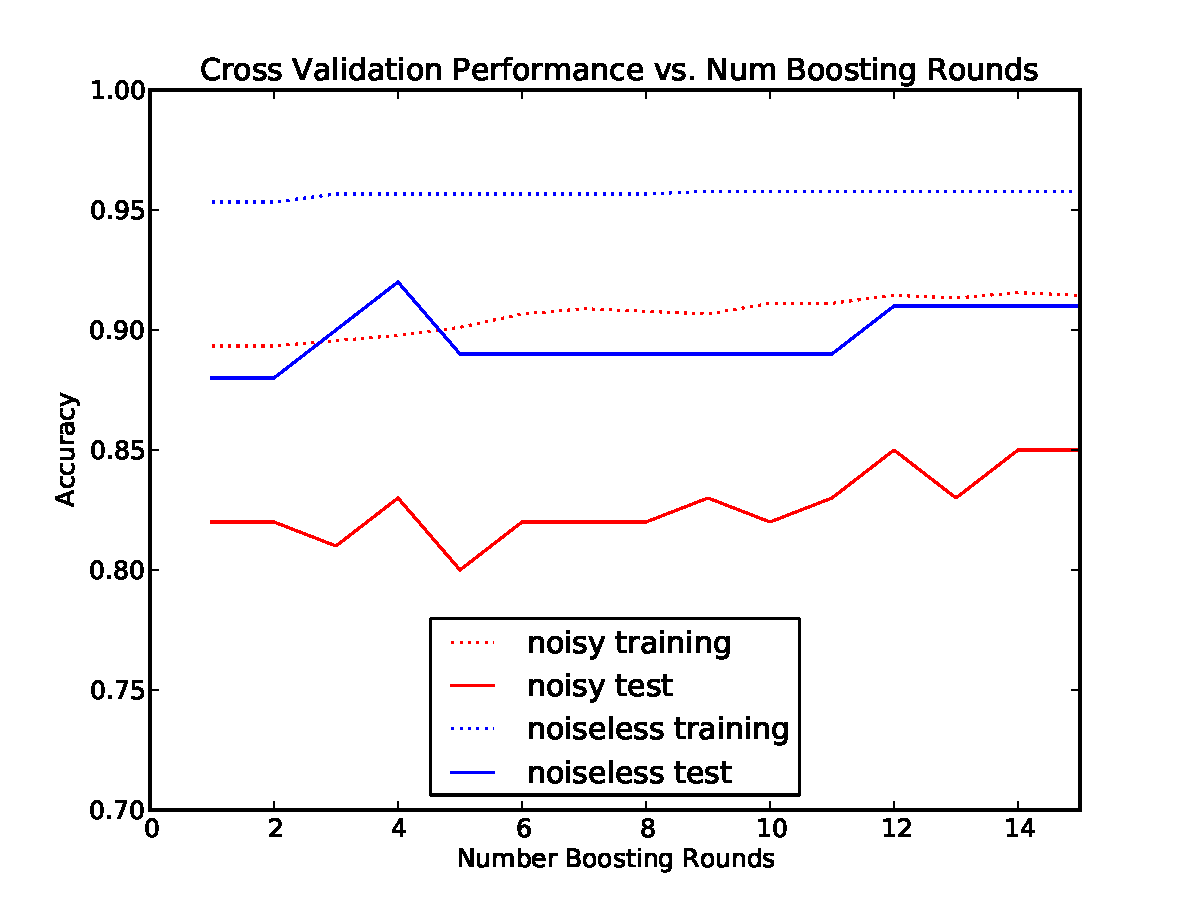
\includegraphics[width=150mm]{nguyen-ming-3D.pdf}$$\\
			This is expected based on our theoretical discussion of boosting in class because
			\item Comparing cross-validated test performance of boosting with ID3 with/without pruning. 
			\begin{itemize}
			\item Comparing performance of boosting with ID3 without pruning, we see that the original ID3 without pruning has an average cross-validated training performance of 0.87 on noiseless test data. This is less than the average 0.90 of the performance of the boosting on a depth 1 tree over [1,15] rounds on the noiseless data. It has a maximum of 0.92. It makes sense that the ID3 algorithm without boosting or pruning would not have a performance that was as good as the modified algorithm.
			\item Looking at the ID3 with pruning we see that there is a mean of 0.874 for non-noisy data over all validation set sizes [1, 80]with a maximum of 0.92. Though these numbers do not correlate exactly for comparision, for purposes of this discussion, the peaks are greater than the original ID3 without pruning or boosting. However, it is equal to the maximum of the boosting performance.
			\end{itemize}
			\item Comparing cross-validated training and test performance for boosting with weak learners of depth 1 over a number of rounds in [1, 15].\\
			(graph)\\
			\item Comparing cross-validated training and test performance for boosting with weak learners of depth 1 over a number of rounds in [1, 15].
<<<<<<< HEAD
			$$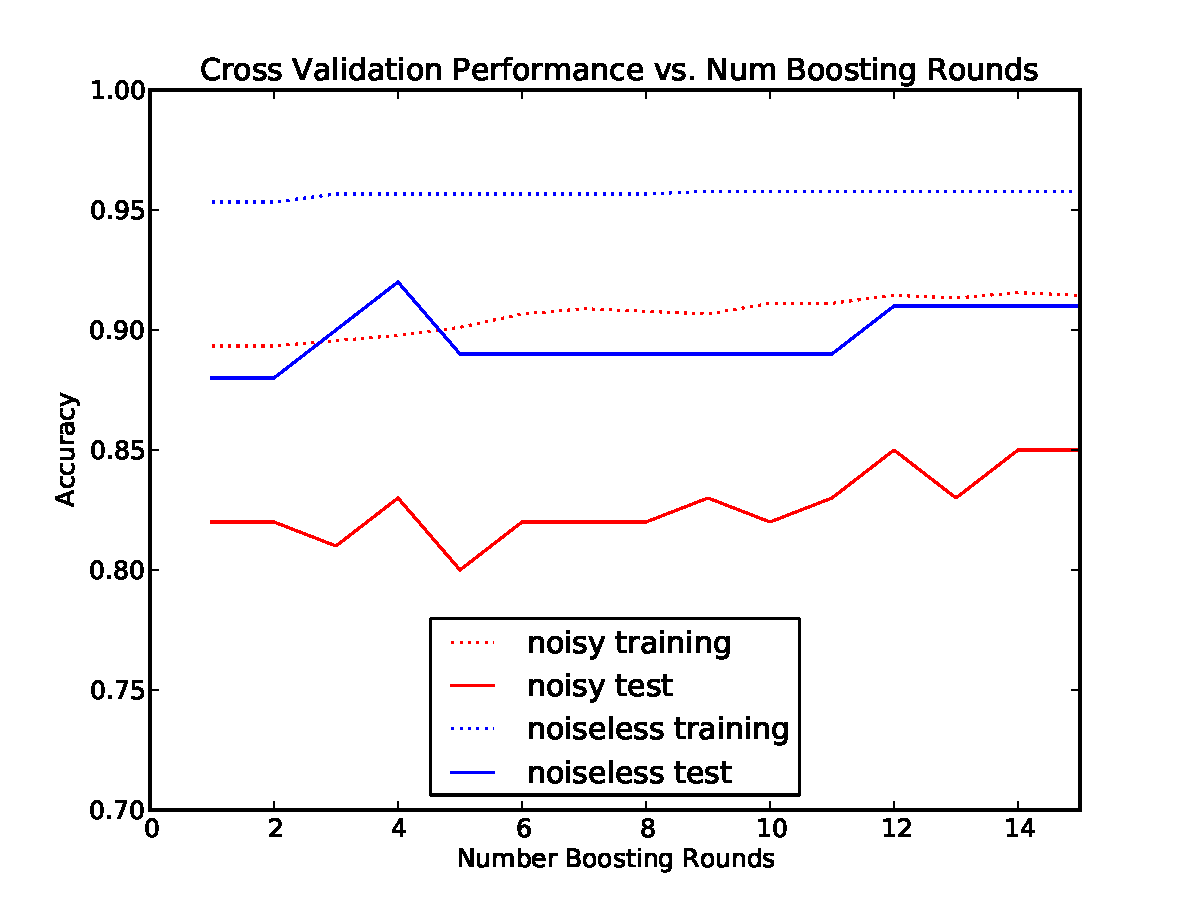
\includegraphics[width=150mm]{nguyen-ming-3D.pdf}$$
			Training and test performance seem to be closely related in that performance for both over increasing number of rounds seem to move in very similar patterns. However the test data seems to show changes to more of an extreme than training data, 
=======
			$$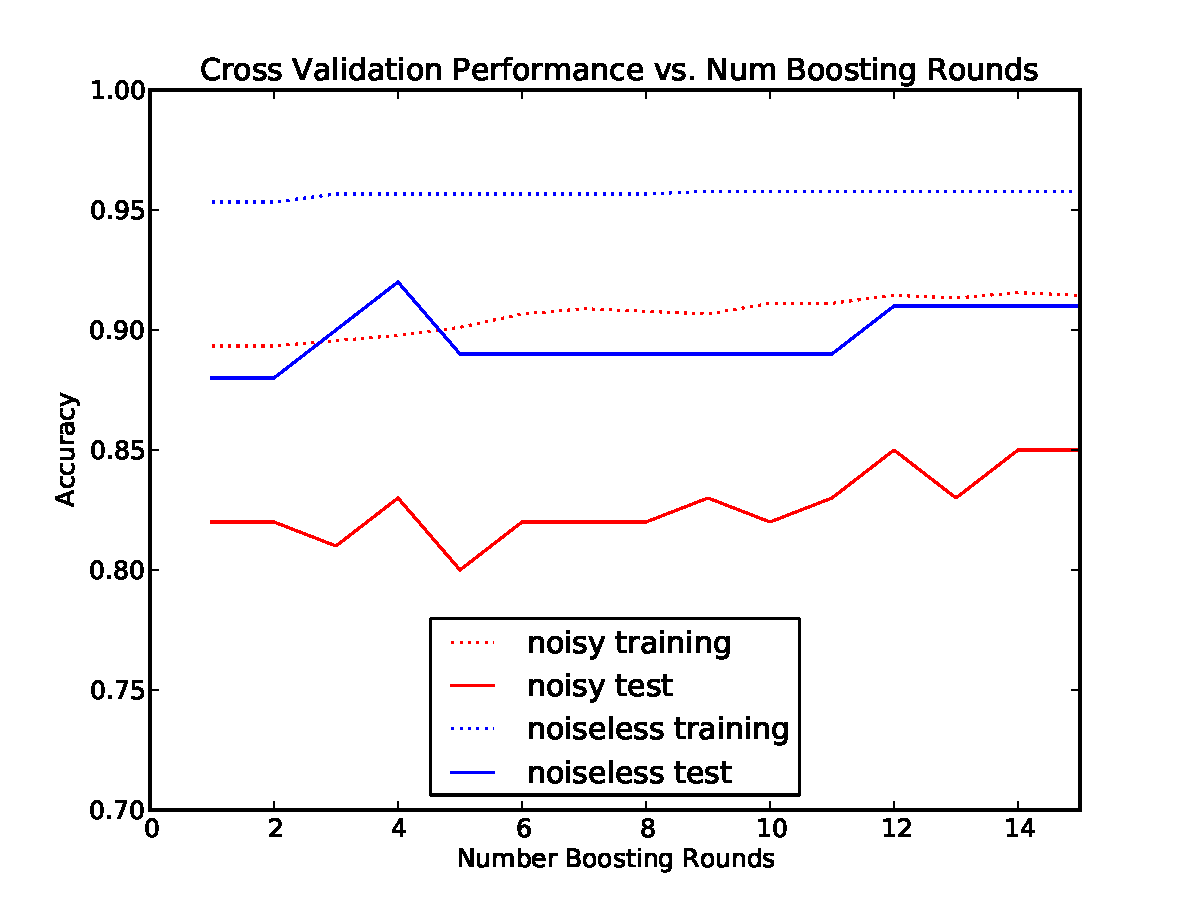
\includegraphics[width=150mm]{nguyen-ming-3D.pdf}$$\\
			The relationship between training and test performance shows that
>>>>>>> dba91106a02e224afa7b35c61ba54ed9d3629e28
		\end{enumerate}
	\end{enumerate}
\end{enumerate}

\item Tree Analysis
$$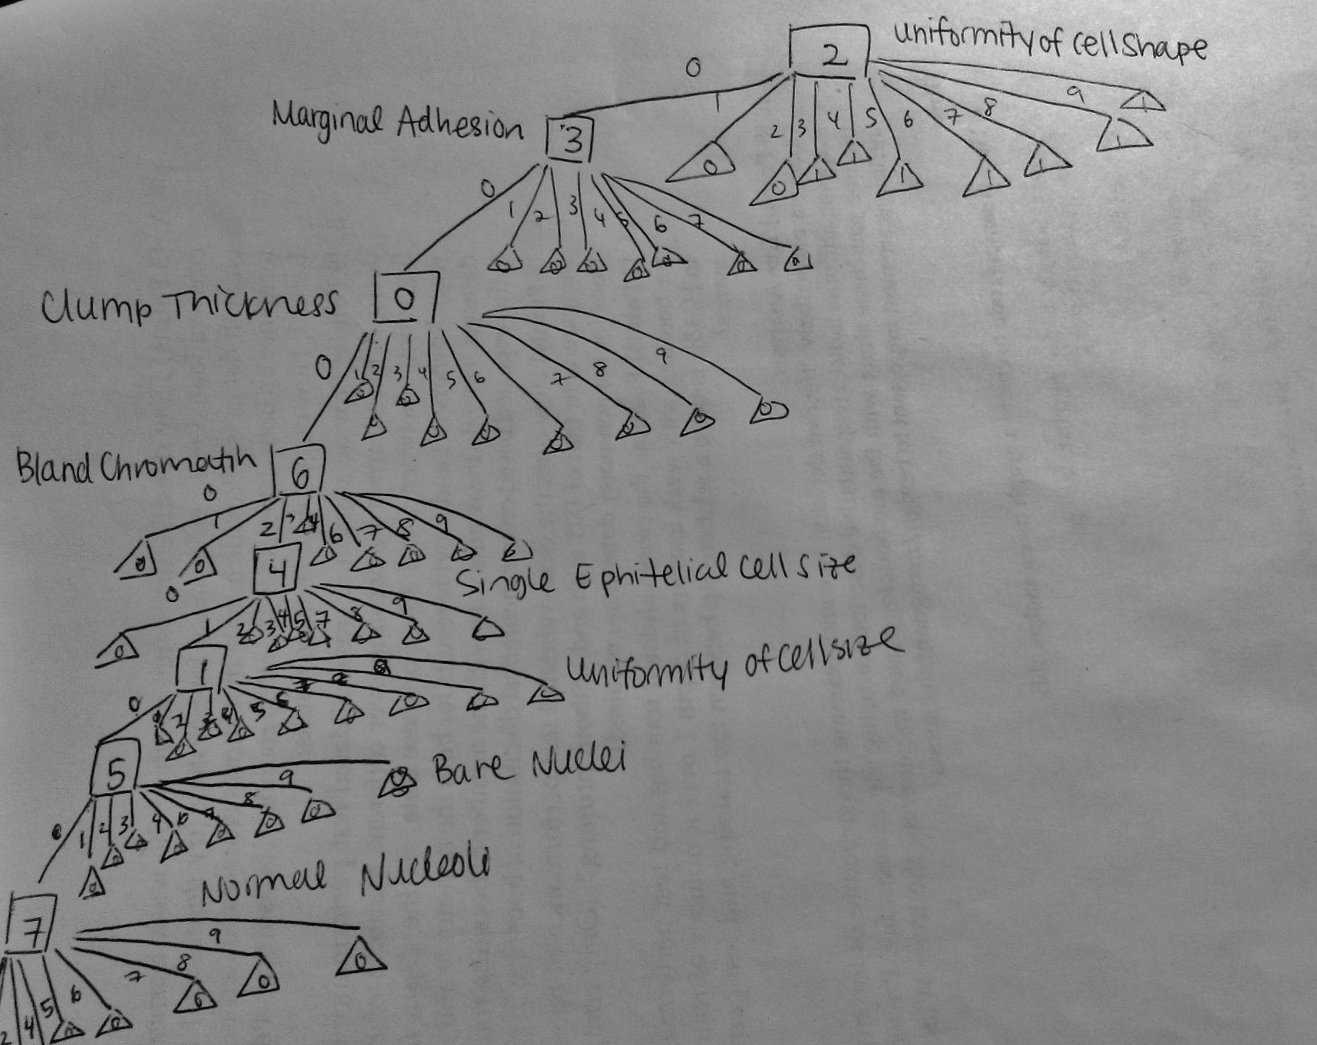
\includegraphics[width=150mm]{p4.jpg}$$
\\ This is one of our most effective decision trees, generated by pruning the original tree with a validation size of 20 and using the first tree resulting from 10-fold cross validation. Its accuracy performance on the test data was 0.9, and its accuracy on the training data was 0.9155. The most important attributes in order of importance for classifying benign/malignant based on this tree are: uniformity of cell shape (attribute 4), marginal adhesion (attribute 5), clump thickness (attribute 2), bland chromatin (attribute 8), single ephitelial cell size (atribute 6), uniformity of cell state (attribute 3), bare nuclei (attribute 7) and normal nucleoli (attribute 9).
\\ We chose this tree based on its performance on the noiseless test set. Overall, decision trees of validation size 20 had the best performance on the test data.
% \begin{enumerate}
% \end{enumerate}

\end{enumerate}
\end{document}